\[ R(t) = 2 + 5 \sin{\frac{4 \pi t}{25}}, \enspace S(t) = \frac{15t}{1 + 3t} \]
\[ A(t) = \textnormal{Total rate} = S(t) - R(t) \]
\subsection{Part A}
We can integrate the loss function to obtain the amount removed over 6 hours like so:
\[ \int_{0}^{6} R(t) \approx 6.723 \enspace yd^3 \]
\subsection{Part B}
We can simply integrate the total rate over time and add it to the initial condition:
\[ Y(t) = \int_{0}^{t} A(x) \, dx + 2500 \]
\subsection{Part C}
We evaluate $A(t)$ at the time point, because that's the total rate:
\[ A(4.0) \approx 1.908 \enspace yd^3 \]
\subsection{Part D}
It's intuitive to look at the graph of $A(t)$:
\begin{center}
	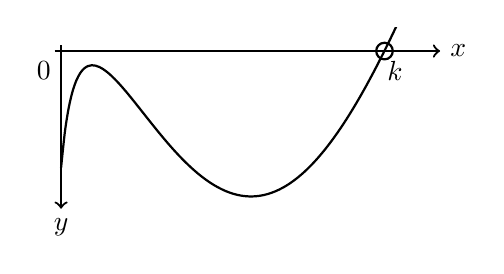
\begin{tikzpicture}
		\begin{axis}[thick,smooth,no markers, hide axis, height=4.4cm, width=8.0cm, ymin=-3.4, ymax=0.4, xmin=-1.0, xmax=7.0]
			\addplot+[black, samples=100, domain=0:6.0] {((15*x)/(1 + (3 * x))) - (2 + (5 * sin(((4 * pi * x)/(25)) r)))};
			\draw[arrows=->, thick] (axis cs:-0.1,0) -- (axis cs:6.0,0) node[right] {$x$};
			\draw[arrows=->, thick] (axis cs:0,0.1) -- (axis cs:0,-2.7) node[below] {$y$};
			\node[below left] at (axis cs:0, 0) {$0$};
			\node[below right] at (axis cs:5.0, 0) {$k$};
			\draw (axis cs:5.12, 0) circle (3pt);
		\end{axis} 
	\end{tikzpicture}
\end{center}
At point $k$, $A(t)$ intersects the x axis. Up until then, the amount of total sand has been decreasing (because $A(t)$ is below the x xis), and at $k$ it has been decreasing the longest. We can no integrate $A(t)$ from $0$ to $k$ to obtain the total amount of sand at that point:
\[ Y(k) \approx 2492.37 \enspace yd^3 \]
